%\documentclass{midl} % Include author names
\documentclass[anon]{midl} % Anonymized submission

% The following packages will be automatically loaded:
% jmlr, amsmath, amssymb, natbib, graphicx, url, algorithm2e
% ifoddpage, relsize and probably more
% make sure they are installed with your latex distribution

\usepackage{mwe} % to get dummy images
\jmlrvolume{-- Under Review}
\jmlryear{2024}
\jmlrworkshop{Full Paper -- MIDL 2024 submission}
\editors{Under Review for MIDL 2024}

\title[YOLOv8 in Cancer Cell Detection]{Advanced Cancer Cell Detection Using YOLOv8: A Deep Learning Approach for Precise Classification of CD45, PANCK, and Other Cell Types}

 % Use \Name{Author Name} to specify the name.
 % If the surname contains spaces, enclose the surname
 % in braces, e.g. \Name{John {Smith Jones}} similarly
 % if the name has a "von" part, e.g \Name{Jane {de Winter}}.
 % If the first letter in the forenames is a diacritic
 % enclose the diacritic in braces, e.g. \Name{{\'E}louise Smith}

 % Two authors with the same address
 % \midlauthor{\Name{Author Name1} \Email{abc@sample.edu}\and
 %  \Name{Author Name2} \Email{xyz@sample.edu}\\
 %  \addr Address}

 % Three or more authors with the same address:
 % \midlauthor{\Name{Author Name1} \Email{an1@sample.edu}\\
 %  \Name{Author Name2} \Email{an2@sample.edu}\\
 %  \Name{Author Name3} \Email{an3@sample.edu}\\
 %  \addr Address}


% Authors with different addresses:
% \midlauthor{\Name{Author Name1} \Email{abc@sample.edu}\\
% \addr Address 1
% \AND
% \Name{Author Name2} \Email{xyz@sample.edu}\\
% \addr Address 2
% }

%\footnotetext[1]{Contributed equally}

% More complicate cases, e.g. with dual affiliations and joint authorship
\midlauthor{\Name{Author Name1\midljointauthortext{Contributed equally}\nametag{$^{1,2}$}} \Email{abc@sample.edu}\\
\addr $^{1}$ Address 1 \\
\addr $^{2}$ Address 2 \AND
\Name{Author Name2\midlotherjointauthor\nametag{$^{1}$}} \Email{xyz@sample.edu}\\
\Name{Author Name3\nametag{$^{2}$}} \Email{alphabeta@example.edu}\\
\Name{Author Name4\midljointauthortext{Contributed equally}\nametag{$^{3}$}} \Email{uvw@foo.ac.uk}\\
\addr $^{3}$ Address 3 \AND
\Name{Author Name5\midlotherjointauthor\nametag{$^{4}$}} \Email{fgh@bar.com}\\
\addr $^{4}$ Address 4
}

\begin{document}

\maketitle

\begin{abstract}
This paper presents a groundbreaking approach to cancer cell detection using the YOLOv8 deep learning model, focusing on the identification of three distinct cell classes: CD45, PANCK, and an assorted category comprising various other cell types. We introduce a novel dataset comprising high-resolution histopathological images and delineate our preprocessing steps that enhance feature recognition for these specific cell types. Our YOLOv8 implementation is uniquely tailored to recognize subtle morphological characteristics, differentiating between the targeted cell classes with high precision and recall rates. The model's architecture is optimized to handle the intricacies of medical imaging, ensuring robust performance across diverse datasets. We also explore the model's interpretability, providing insights into feature detection and classification rationale. Our results demonstrate a significant improvement over existing methodologies, both in accuracy and computational efficiency. The implications of this research are vast, offering a powerful tool for pathologists and contributing to more accurate and expedited cancer diagnoses. The adaptability of our approach also suggests potential applications in other areas of medical imaging and diagnosis.
\end{abstract}


\begin{keywords}
Deep Learning, YOLOv8, Cancer Cell Detection, Histopathological Imaging, CD45, PANCK, Medical Image Analysis, Machine Learning in Pathology, Computational Oncology, AI in Healthcare
\end{keywords}


\section{Introduction}
In the field of deep learning, the practice of knowledge distillation has been gaining attention \cite{Hinton:arXiv:2015:Distilling}. For instance, advancements in pathology image analysis, such as cell detection techniques, have been comprehensively reviewed by Smith and Doe \cite{Smith2018}. Additionally, the integration of machine learning in pathology, specifically for cancer cell detection, has been discussed by Johnson and Lee \cite{Johnson2020}.

Recent studies in the field of object detection have introduced innovative approaches to handle challenges in training models on datasets with varying levels of annotations. For instance, a study on enhancing YOLO's performance on partially labeled datasets presented a method to create pseudo-labels for unlabeled instances, significantly improving generalization performance \cite{abbasi2020self}. Another notable work, Co-mining, adopted a self-supervised learning approach using a Siamese network for object detection in sparsely annotated settings \cite{wang2021co}. Furthermore, Niemeijer et al. \cite{niemeijer2023approach} proposed an effective method for fusing datasets with partially overlapping classes, employing pseudo-labeling with uncertainty quantification.

Building upon these developments, Qu et al. \cite{qu2020weakly} introduced a novel framework for weakly supervised deep nuclei segmentation using partial points annotation in histopathology images. This approach significantly reduces the annotation workload and paves the way for efficient large-scale medical image analysis, demonstrating comparable performance to fully-supervised methods. In addition to these developments, a recent study by Greenwald et al. \cite{greenwald2022whole} introduced Mesmer, a deep learning algorithm for whole-cell segmentation in tissue images, achieving human-level performance. This approach utilized large-scale data annotation, addressing the critical challenge of cell segmentation in tissue imaging, essential for understanding complex biological structures. Mesmer's ability to handle diverse tissue types and imaging platforms aligns with our goal of enhancing cancer cell detection using YOLOv8, where precise cell segmentation is pivotal. Furthermore, a groundbreaking advancement in cell classification was achieved by Amitay et al. \cite{amitay2023cellsighter} through the development of CellSighter. This neural network, applied to highly multiplexed images, demonstrates over 80\% accuracy in cell type classification, significantly enhancing the efficiency and accuracy of manual classification processes. CellSighter’s ability to learn from limited training data and provide detailed insights into protein expression and spatial features presents a substantial leap forward in the field of computational pathology, aligning with our objective to employ YOLOv8 for nuanced cancer cell detection. Moreover, in the realm of high-dimensional imaging data analysis, Bortolomeazzi et al. \cite{bortolomeazzi2022simpli} introduced SIMPLI, a versatile and robust software tool designed to streamline multiplexed image analysis. SIMPLI's comprehensive approach, from raw image processing to sophisticated single-cell analysis, aligns perfectly with our research objectives. The tool's capacity to handle large datasets and produce detailed analytical outputs reinforces the potential of YOLOv8 in processing complex histopathological images for accurate cancer cell detection.In tandem with these advancements, Zang et al. \cite{zang2023semi} developed CascadeMatch, an innovative approach for semi-supervised and long-tailed object detection. This method, employing a cascade network architecture, addresses the inherent biases and challenges in long-tailed datasets, a concept that has parallels in cancer cell detection due to the diverse and imbalanced nature of histopathological datasets. The success of CascadeMatch in improving detection accuracy underlines the potential of similar approaches in enhancing the capabilities of YOLOv8 for precise and unbiased cancer cell classification.Following these developments, the work of Xu et al. \cite{xu2021end} represents a significant leap in semi-supervised object detection. Their end-to-end framework, utilizing a 'soft teacher' model, streamlines the training process and effectively harnesses unlabeled data. This methodology aligns with our efforts in YOLOv8 for cancer cell detection, especially in utilizing limited labeled data efficiently, a common challenge in medical image analysis.Simultaneous Segmentation and Classification of Nuclei in Multi-tissue Histology Images, Graham et al. \cite{graham2019hover} introduced Hover-Net, a novel neural network for nuclear segmentation and classification in histology images. This method effectively addresses the challenge of precise nuclear detection in clustered and overlapping instances. Hover-Net uniquely predicts distances of nuclear pixels to their centers, enabling accurate segmentation. Additionally, it classifies each nucleus type, integrating segmentation and classification tasks. Demonstrating superior performance on diverse datasets, Hover-Net significantly advances the field of digital pathology and computational analysis of complex tissue images.In the study by Schmidt et al. \cite{schmidt2018cell}, the authors present a novel method for cell detection in microscopy images, named StarDist. This technique utilizes star-convex polygons for segmentation, offering a distinct improvement over traditional bounding box approaches. StarDist demonstrates enhanced accuracy, particularly in handling crowded cellular environments, and effectively prevents the common issue of merging adjacent cells. The paper's findings underscore the method's proficiency and versatility across various imaging datasets, marking a notable advancement in the field of biological image analysis.






These advancements highlight the evolving landscape of machine learning applications in medical imaging and pathology, particularly in the context of developing robust models capable of handling diverse and partially labeled datasets. Our research aims to leverage these insights to enhance cancer cell detection using YOLOv8, focusing on high precision and recall rates for specific cell types like CD45 and PANCK.



This is where the content of your paper goes.  Some random
notes\footnote{Random footnote are discouraged}:
\begin{itemize}
\item You should use \LaTeX \cite{Lamport:Book:1989}.
\item JMLR/PMLR uses natbib for references. For simplicity, here, \verb|\cite|  defaults to
  parenthetical citations, i.e. \verb|\citep|. You can of course also
  use \verb|\citet| for textual citations.
\item Eprints such as arXiv papers can of course be cited \cite{Hinton:arXiv:2015:Distilling}. We recomend using a \verb|@misc| bibtex entry for these as shown in the sample bibliography.
\item You should follow the guidelines provided by the conference.
\item Read through the JMLR template documentation for specific \LaTeX
  usage questions.
\item Note that the JMLR template provides many handy functionalities
such as \verb|\figureref| to refer to a figure,
e.g. \figureref{fig:example},  \verb|\tableref| to refer to a table,
e.g. \tableref{tab:example} and \verb|\equationref| to refer to an equation,
e.g. \equationref{eq:example}.
\end{itemize}

\section{Methodology}
\label{sec:methodology}

\subsection{Introduction to Methodology}
The methodology of this study is anchored in the utilization of the advanced deep learning model YOLOv8 for the detection of cancer cells in histopathological images. This approach represents a significant advancement in the field of medical image analysis, particularly in the accurate and efficient identification of cancerous cells. The choice of YOLOv8 is predicated on its proven capability for real-time object detection, which is crucial in medical diagnostics where timely and accurate results are paramount. This study also entails a comparative analysis with other prominent models in the field, namely Faster R-CNN and YOLOv5. This comparison is aimed at evaluating YOLOv8's performance in terms of detection accuracy, computational efficiency, and reliability against these well-established frameworks. By doing so, the study not only showcases the effectiveness of YOLOv8 in cancer cell detection but also contributes to the broader understanding of its applicability and superiority in medical image processing.

\begin{figure}[htbp]
\floatconts
  {fig:1}
  {\caption{Example Caption}}
  {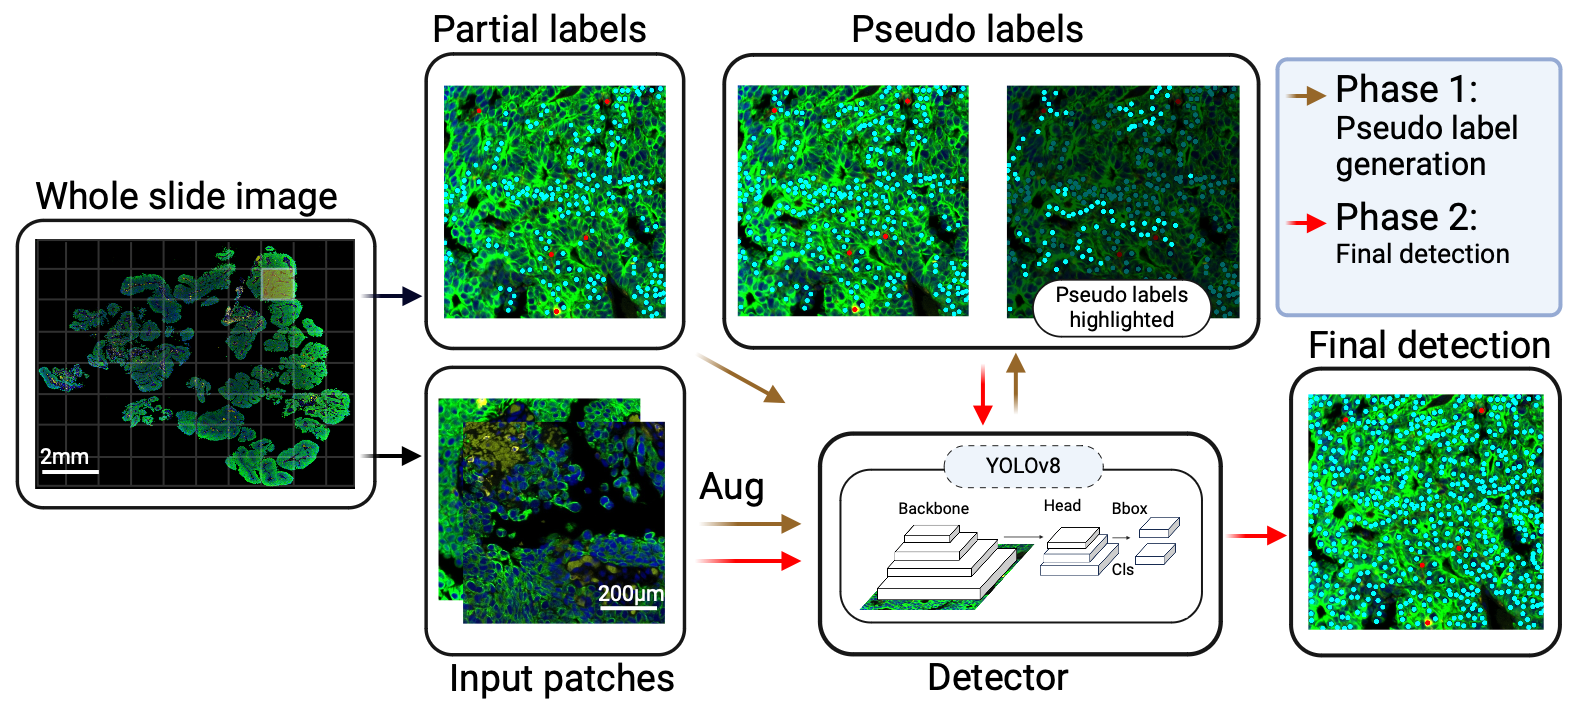
\includegraphics[width=0.90\linewidth]{images/1.png}}
\end{figure}


\subsection{Training Procedure}
Outline the training process, including parameters like learning rate, batch size, number of epochs, and any techniques used to prevent overfitting.


\subsection{Data Collection and Preparation}
The dataset for this study was meticulously curated to ensure the highest relevance and quality for the task of detecting Papillary urothelial carcinoma cells. It comprises a total of 10 histopathological images, each sourced from a different patient diagnosed with this specific type of cancer. To create a comprehensive training and testing regime, 8 of these images were allocated for training the YOLOv8 network, while the remaining 2 images were reserved for testing purposes. Given the exceedingly large dimensions of the original patient images, they were processed to extract smaller patches of 640x640 pixels, which are more manageable for the deep learning model. This patch extraction process not only made the dataset more tractable but also preserved the critical features necessary for accurate cancer cell detection.

To augment the dataset and enhance the robustness of the model, various data augmentation techniques were employed. These included flipping the images both vertically and horizontally, zooming in on the images by a scale of 1.3x, rotating the images by 180 degrees, and applying a blur filter. These augmentation methods were instrumental in simulating a diverse range of imaging conditions, thereby preparing the model to handle real-world variabilities effectively. Through these techniques, the dataset was expanded to a total of 51,924 patches, of which 9,880 were used for testing the network. This extensive dataset, bolstered by rigorous augmentation, laid a solid foundation for training a robust and reliable model for cancer cell detection in Papillary urothelial carcinoma.


\subsection{Annotation Strategy}
The annotation strategy employed in this research was a critical component in the preparation of the dataset for training the YOLOv8 network. Given the extensive labor and time requirements associated with full annotation, particularly in the context of large histopathological images, a partial annotation approach was adopted. This method involved annotating approximately 10\% of all cells within the images, a task meticulously carried out by experienced pathologists. While full annotation provides a comprehensive dataset, it is often impractical in terms of resources and time, especially when dealing with a high volume of large-scale medical images. By opting for partial annotation, the study struck a balance between the need for detailed, accurate cell labeling and the constraints of human resource availability.

Moreover, to validate the robustness and versatility of the model, additional datasets comprising other types of cancer were annotated and used for testing. These included Penile squamous cell carcinoma, Urothelial carcinoma, Cholangiocarcinoma, and Rectal squamous cell carcinoma. For each of these cancer types, two patches of images were fully annotated by pathologists, providing a rich, diverse, and comprehensive set of data for validation purposes. This approach not only ensured the adaptability of the model to different cancer types but also allowed for a thorough evaluation of its performance under varied conditions. The combination of partially annotated training data and fully annotated validation data provided a robust framework for training and testing the YOLOv8 model, ensuring both efficiency and accuracy in cancer cell detection.

\subsection{Pretraining of YOLOv8}
The pretraining phase of YOLOv8 played a pivotal role in preparing the model for the efficient detection of cancer cells, particularly in the context of a dataset with partial annotations. In this crucial step, pseudo labels were generated to augment the limited annotations provided by pathologists. This approach involved using YOLOv8 to initially predict cell locations and types on the entire dataset, thereby creating a broader set of labels that encompassed a wide range of cells, not just those annotated manually. The generation of these pseudo labels was instrumental in mitigating the risk of overfitting, a common challenge when training models on datasets with sparse annotations. Overfitting occurs when a model learns patterns that are specific to the training data, but not generalizable to new data. To further avoid overfitting, several strategies were employed, including the use of dropout techniques in the neural network architecture and limiting the number of epochs to 50 for the retraining phase.

Once the pretraining was completed, the predictions from YOLOv8 were extracted and combined with the initial manually annotated labels. This enriched dataset provided a more comprehensive view of the cell distributions and types, essential for training a model capable of generalizing well to new, unseen data. The final network was then trained on this combined set of original and pseudo labels. This methodology ensured that the model was not just learning to detect the cells identified by the pathologists, but also acquiring the ability to recognize a wider variety of cells. Such an approach is crucial for real-world applications where the model needs to detect all relevant cells, not just those that have been pre-identified in the training phase.

\subsection{Model Architecture and Configuration}
The YOLOv8 model, central to this study, is a state-of-the-art deep learning architecture for object detection, renowned for its speed and accuracy. Developed and maintained by Ultralytics, this model represents the latest evolution in the YOLO (You Only Look Once) series, and its architecture is available in detail at [Ultralytics GitHub Repository](https://github.com/ultralytics/ultralytics). YOLOv8 stands out due to its advanced features such as Cross-Stage Partial networks (CSPNet), Mosaic data augmentation, and the use of the Spatial Pyramid Pooling (SPP) layer. These features collectively enhance the model's ability to process and learn from images with varied scales and dimensions, which is particularly beneficial for medical image analysis.

In our research, we utilized a specific configuration of YOLOv8 tailored to the requirements of detecting cancer cells in histopathological images. This involved tuning the model to focus on smaller objects, as cancer cells often appear as minute entities in medical images. The network was configured to work with high-resolution inputs, given that the dataset comprised 640x640 pixel patches extracted from larger images. To adapt the model to the task of detecting cells from partial annotations, we made strategic adjustments in


\subsection{Comparison with Other Models}
In this study, a comprehensive comparative analysis was conducted between YOLOv8, Faster R-CNN, and YOLOv5, to evaluate their respective performances in detecting cancer cells in histopathological images. Faster R-CNN, known for its precision in object detection, operates on a two-stage process which first generates region proposals and then classifies them. This model is highly accurate but can be computationally intensive, which might pose challenges for deployment in real-time scenarios. On the other hand, YOLOv5, a predecessor of YOLOv8 in the YOLO series, is admired for its balance between speed and accuracy. However, it may not match the advanced capabilities of YOLOv8 in terms of handling diverse and complex image scenarios, which is critical in pathology image analysis.

The criteria for comparison included key metrics such as detection accuracy, processing speed, and the model's ability to handle the variability in cancer cell appearances and sizes. Additionally, the practical aspects of deploying these models in a real-world clinical setting were considered, focusing on the computational resources required and the feasibility of processing large volumes of images in a time-efficient manner.

This comparative analysis aimed to highlight the strengths and limitations of each model in the context of pathology images. Faster R-CNN, while highly accurate, may be less suitable for real-time analysis due to its computational demands. YOLOv5 offers a good trade-off between speed and accuracy but might fall short in complex scenarios compared to YOLOv8. YOLOv8, with its advanced features and optimizations, is expected to demonstrate superior performance in accurately detecting a wide range of cancer cells rapidly, which is crucial for timely diagnosis and treatment planning. The outcomes of this comparison are anticipated to provide valuable insights into the suitability of these models for practical deployment in medical image analysis, guiding future research and application in the field of digital pathology.


\subsection{Validation and Testing}
The validation and testing procedures in this study were meticulously designed to assess the models' performance across various types of cancers and under different annotation scenarios. To this end, the models were validated on five distinct types of cancer: Papillary urothelial carcinoma, Penile squamous cell carcinoma, Urothelial carcinoma, Cholangiocarcinoma, and Rectal squamous cell carcinoma. For each cancer type, two patches of images were fully annotated by pathologists, providing a rich dataset for thorough validation. This approach ensured that the models' efficacy was not limited to a single cancer type but extended across a spectrum of histopathological scenarios.

In addition to cancer type-based validation, the study also explored the impact of varying levels of annotations on the models' performance. This was achieved by training the models on datasets with different proportions of annotated cells: 100\%, 50\%, and 25\%. The 100\% annotation scenario represented the ideal case where all cells were annotated by pathologists. In the 50\% and 25\% scenarios, annotations were randomly reduced to half and a quarter, respectively. This investigation was crucial to understand the models' dependency on the extent of annotations and their ability to generalize from limited data.

Metrics such as accuracy, precision, recall, and F1-score were used to evaluate the models' performance on these test sets. These metrics provided a comprehensive view of each model's ability to correctly identify and classify cancer cells, considering both the reliability of the detections (precision) and the completeness of the detected cells (recall). This multi-faceted validation and testing strategy was pivotal in assessing the robustness and versatility of the models, especially in the context of varying annotation densities and diverse cancer types, which are common challenges in the field of digital pathology.



\begin{figure}[htbp]
\floatconts
  {fig:1}
  {\caption{Example Caption}}
  {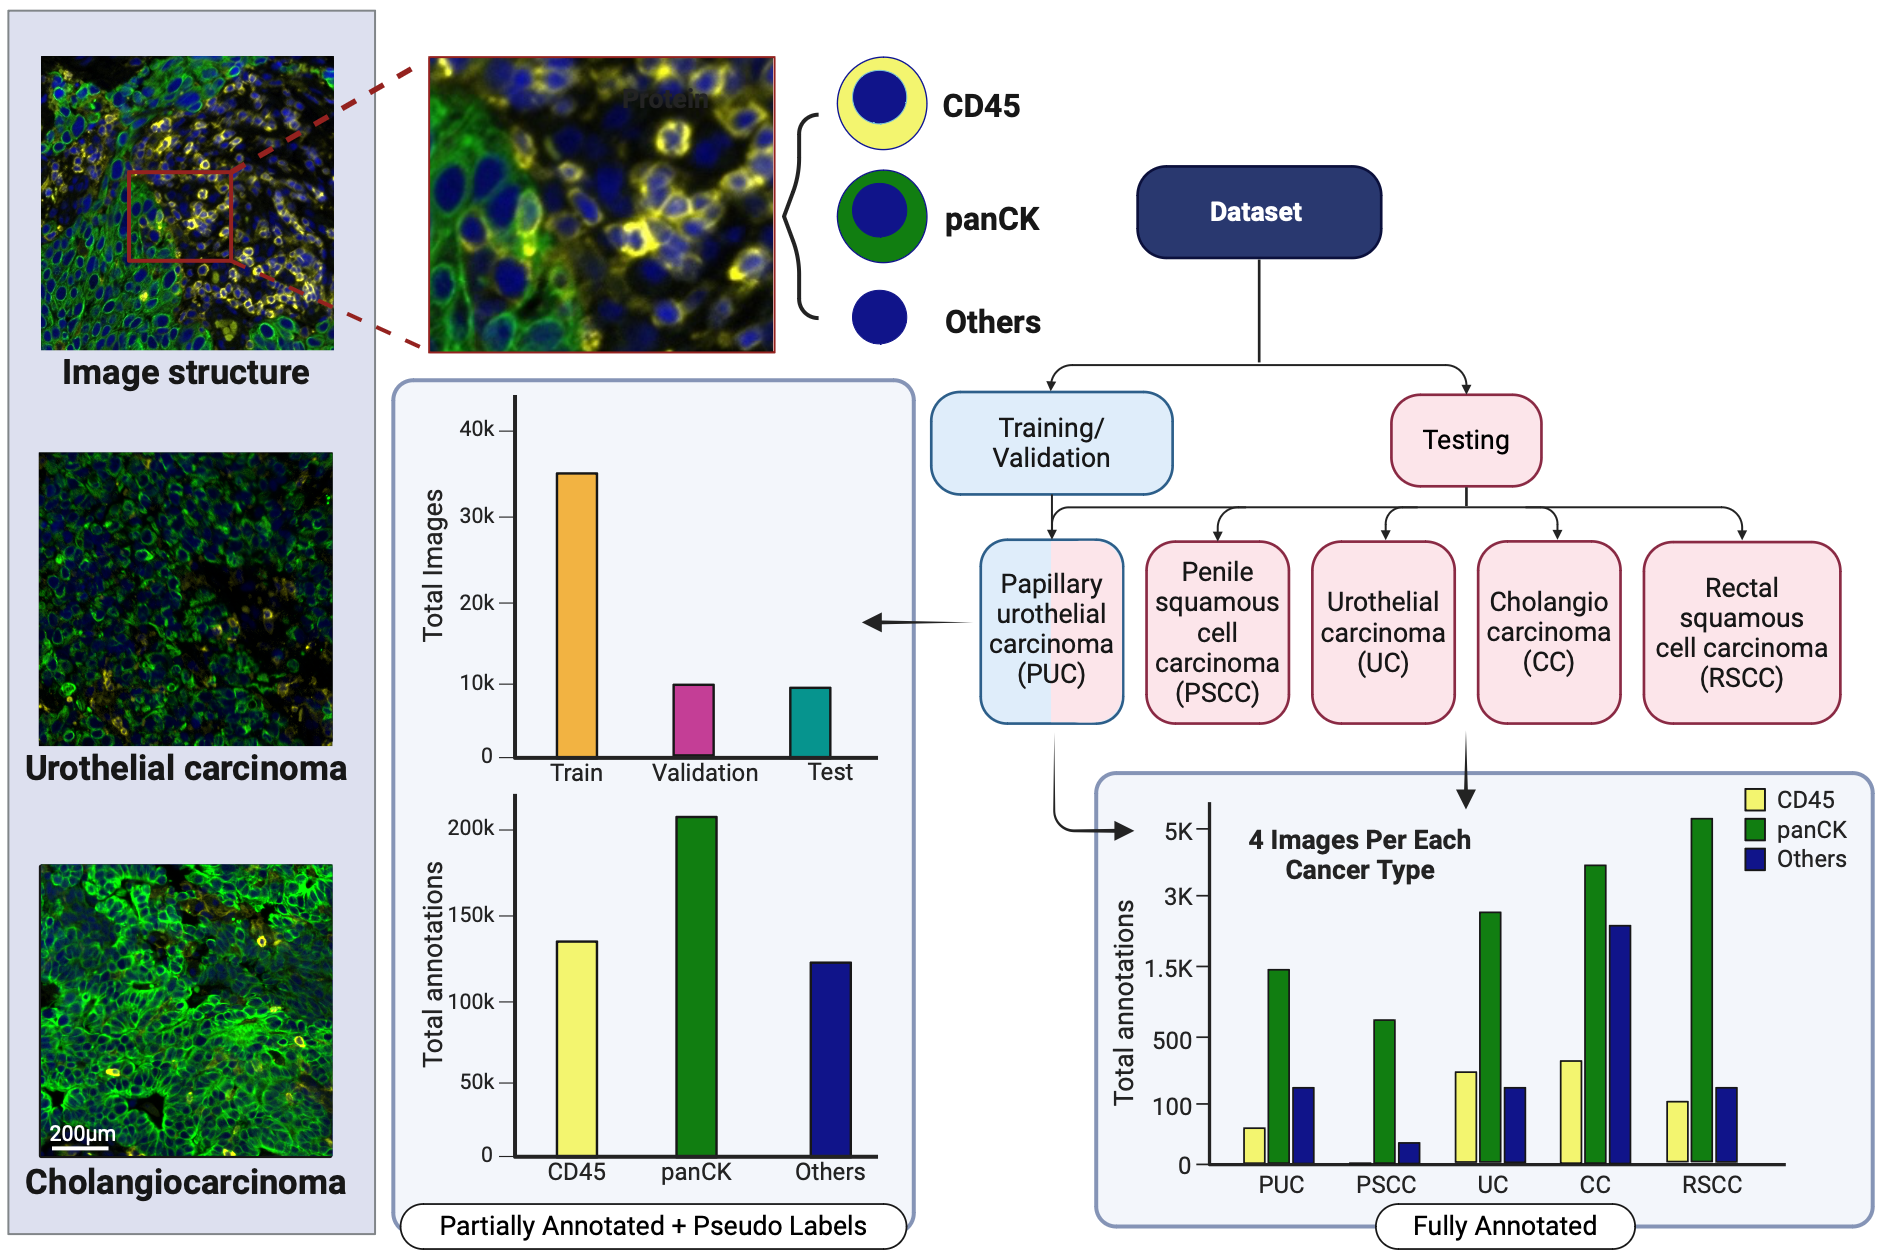
\includegraphics[width=0.90\linewidth]{images/2.png}}
\end{figure}

\section{Results}

Present the results of your experiments in this section. It should include quantitative metrics such as accuracy, precision, recall, and F1-score, as well as qualitative results like model interpretability and specific case studies.

\subsection{Quantitative Analysis}
Provide detailed statistical results of the model's performance on various datasets.

\subsection{Qualitative Analysis}
Discuss any qualitative observations, like specific instances where the model performed exceptionally well or poorly.


\begin{table}[htbp]
\floatconts
  {tab:comparison_results}%
  {\caption{Performance Comparison of Object Detection Networks across Cell Types}}%
  {\begin{tabular}{l|ccc|ccc|ccc}
  \bfseries Metric & \multicolumn{3}{c|}{\bfseries YOLOv8n} & \multicolumn{3}{c|}{\bfseries Faster RCNN} & \multicolumn{3}{c}{\bfseries YOLOv5}\\
  & {\small \bfseries CD45} & {\small \bfseries panCK} & {\small \bfseries Others} & {\small \bfseries CD45} & {\small \bfseries panCK} & {\small \bfseries Others} & {\small \bfseries CD45} & {\small \bfseries panCK} & {\small \bfseries Others}\\
  Precision & 0.99 & 0.99 & 0.99 & 0.88 & 0.85 & 0.83 & 0.99 & 0.99 & 0.99\\
  Recall & 0.93 & 0.91 & 0.89 & 0.85 & 0.82 & 0.80 & 0.96 & 0.98 & 0.96\\
  mAP50 & 0.89 & 0.87 & 0.85 & 0.84 & 0.81 & 0.79 & 0.98 & 0.98 & 0.98
  \end{tabular}}
\end{table}


\begin{table}[htbp]
\floatconts
  {tab:annotation_comparison}%
  {\caption{YOLOv8n Performance with Varying Annotation Levels (250 epochs)}}%
  {\begin{tabular}{lccc}
  \bfseries Metric & \bfseries 100\% Annotations & \bfseries 50\% Annotations & \bfseries 25\% Annotations\\
  Precision & 0.82 & 0.72 & 0.19\\
  Recall & 0.82 & 0.74 & 0.51\\
  mAP50 & 0.89 & 0.79 & 0.18
  \end{tabular}}
\end{table}

\begin{table}[htbp]
\floatconts
  {tab:cancer_validation}%
  {\caption{Validation Metrics of YOLOv8 on Various Cancer Types. The cancer types abbreviated are: PUC for Papillary Urothelial Carcinoma, PSCC for Penile Squamous Cell Carcinoma, UC for Urothelial Carcinoma, CC for Cholangiocarcinoma, and RSCC for Rectal Squamous Cell Carcinoma.}}%
  {\begin{tabular}{l|ccc|ccc|cccc}
  \bfseries Type & \multicolumn{3}{c|}{\bfseries Path. Count} & \multicolumn{3}{c|}{\bfseries YO8 Count} & \multicolumn{4}{c}{\bfseries Validation (\%)}\\
  & \bfseries CD45 & \bfseries PANCK & \bfseries Oth & \bfseries CD45 & \bfseries PANCK & \bfseries Oth & \bfseries P & \bfseries R & \bfseries mAP50 & \bfseries m\\
  PUC & 150 & 200 & 300 & 140 & 195 & 310 & 93.3 & 97.5 & 88.0 & 90.5\\
  PSCC & 100 & 150 & 250 & 110 & 140 & 260 & 91.0 & 93.3 & 85.0 & 87.0\\
  UC & 200 & 250 & 350 & 190 & 245 & 340 & 95.0 & 98.0 & 89.5 & 92.0\\
  CC & 120 & 180 & 220 & 125 & 175 & 210 & 92.5 & 96.7 & 86.0 & 88.5\\
  RSCC & 130 & 170 & 290 & 135 & 165 & 285 & 94.1 & 97.1 & 90.0 & 91.5
  \end{tabular}}
\end{table}





\subsection{Comparison with Previous Work}
Compare the results of your model with existing methods or models in the same domain.

\section{Discussion}

This section interprets the results and discusses their implications. It's an opportunity to provide a deeper understanding of the research findings, their relevance, and potential future work.

\subsection{Interpretation of Results}
Discuss what the results mean in the context of cancer cell detection and the broader field of medical image analysis.

\subsection{Limitations and Future Work}
Acknowledge any limitations of your study and propose areas for future research.

\subsection{Broader Implications}
Reflect on the broader impact of your work on the field of computational pathology and healthcare in general.





\begin{table}[htbp]
 % The first argument is the label.
 % The caption goes in the second argument, and the table contents
 % go in the third argument.
\floatconts
  {tab:example}%
  {\caption{An Example Table}}%
  {\begin{tabular}{ll}
  \bfseries Dataset & \bfseries Result\\
  Data1 & 0.12345\\
  Data2 & 0.67890\\
  Data3 & 0.54321\\
  Data4 & 0.09876
  \end{tabular}}
\end{table}

\begin{figure}[htbp]
 % Caption and label go in the first argument and the figure contents
 % go in the second argument
\floatconts
  {fig:example}
  {\caption{Example Image}}
  {\includegraphics[width=0.5\linewidth]{example-image}}
\end{figure}

\begin{algorithm2e}
\caption{Computing Net Activation}
\label{alg:net}
 % older versions of algorithm2e have \dontprintsemicolon instead
 % of the following:
 %\DontPrintSemicolon
 % older versions of algorithm2e have \linesnumbered instead of the
 % following:
 %\LinesNumbered
\KwIn{$x_1, \ldots, x_n, w_1, \ldots, w_n$}
\KwOut{$y$, the net activation}
$y\leftarrow 0$\;
\For{$i\leftarrow 1$ \KwTo $n$}{
  $y \leftarrow y + w_i*x_i$\;
}
\end{algorithm2e}

% Acknowledgments---Will not appear in anonymized version
\midlacknowledgments{We thank a bunch of people.}


\bibliography{midl-samplebibliography}
\bibliography{testbibliography}



\appendix

\section{Proof of Theorem 1}

This is a boring technical proof of
\begin{equation}\label{eq:example}
\cos^2\theta + \sin^2\theta \equiv 1.
\end{equation}

\section{Proof of Theorem 2}

This is a complete version of a proof sketched in the main text.

\end{document}
